\documentclass[14pt]{extbook}
\usepackage{multicol, enumerate, enumitem, hyperref, color, soul, setspace, parskip, fancyhdr} %General Packages
\usepackage{amssymb, amsthm, amsmath, bbm, latexsym, units, mathtools} %Math Packages
\everymath{\displaystyle} %All math in Display Style
% Packages with additional options
\usepackage[headsep=0.5cm,headheight=12pt, left=1 in,right= 1 in,top= 1 in,bottom= 1 in]{geometry}
\usepackage[usenames,dvipsnames]{xcolor}
\usepackage{dashrule}  % Package to use the command below to create lines between items
\newcommand{\litem}[1]{\item#1\hspace*{-1cm}\rule{\textwidth}{0.4pt}}
\pagestyle{fancy}
\lhead{Makeup Progress Quiz -1}
\chead{}
\rhead{Version B}
\lfoot{7547-2949}
\cfoot{}
\rfoot{Fall 2020}
\begin{document}

\begin{enumerate}
\litem{
Determine the horizontal and/or oblique asymptotes in the rational function below.\[ f(x) = \frac{8x^{3} +14 x^{2} -7 x -15}{2x^{2} -3 x -9} \]\begin{enumerate}[label=\Alph*.]
\item \( \text{Horizontal Asymptote of } y = 4.0  \)
\item \( \text{Horizontal Asymptote of } y = 3.0 \text{ and Oblique Asymptote of } y = 4x + 13 \)
\item \( \text{Horizontal Asymptote at } y = 3.0 \)
\item \( \text{Horizontal Asymptote of } y = 4.0 \text{ and Oblique Asymptote of } y = 4x + 13 \)
\item \( \text{Oblique Asymptote of } y = 4x + 13. \)

\end{enumerate} }
\litem{
Determine the horizontal and/or oblique asymptotes in the rational function below.\[ f(x) = \frac{6x^{2} +19 x -20}{30x^{3} -133 x^{2} +144 x -45} \]\begin{enumerate}[label=\Alph*.]
\item \( \text{Oblique Asymptote of } y = 5x -38. \)
\item \( \text{Horizontal Asymptote of } y = 0 \)
\item \( \text{Horizontal Asymptote at } y = -4.000 \)
\item \( \text{Horizontal Asymptote of } y = 0.200 \text{ and Oblique Asymptote of } y = 5x -38 \)
\item \( \text{Horizontal Asymptote of } y = 0.200  \)

\end{enumerate} }
\litem{
Which of the following functions \textit{could} be the graph below?
\begin{center}
    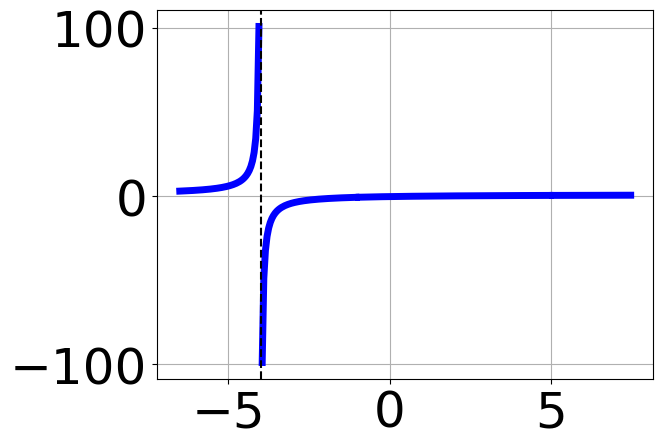
\includegraphics[width=0.5\textwidth]{../Figures/identifyGraphOfRationalFunctionB.png}
\end{center}
\begin{enumerate}[label=\Alph*.]
\item \( f(x)=\frac{x^{3} +8 x^{2} +5 x -14}{x^{3} -21 x -20} \)
\item \( f(x)=\frac{x^{3} +5 x^{2} -x -5}{x^{3} -21 x + 20} \)
\item \( f(x)=\frac{x^{3} +5 x^{2} -x -5}{x^{3} -21 x + 20} \)
\item \( f(x)=\frac{x^{3} -5 x^{2} -x + 5}{x^{3} -21 x -20} \)
\item \( \text{None of the above are possible equations for the graph.} \)

\end{enumerate} }
\litem{
Determine the horizontal and/or oblique asymptotes in the rational function below.\[ f(x) = \frac{6x^{3} +31 x^{2} +8 x -80}{3x^{2} +8 x -16} \]\begin{enumerate}[label=\Alph*.]
\item \( \text{Horizontal Asymptote of } y = 2.0  \)
\item \( \text{Horizontal Asymptote of } y = -4.0 \text{ and Oblique Asymptote of } y = 2x + 5 \)
\item \( \text{Oblique Asymptote of } y = 2x + 5. \)
\item \( \text{Horizontal Asymptote of } y = 2.0 \text{ and Oblique Asymptote of } y = 2x + 5 \)
\item \( \text{Horizontal Asymptote at } y = -4.0 \)

\end{enumerate} }
\litem{
Determine the vertical asymptotes and holes in the rational function below.\[ f(x) = \frac{6x^{3} -13 x^{2} -9 x + 10}{9x^{2} -18 x + 8} \]\begin{enumerate}[label=\Alph*.]
\item \( \text{Vertical Asymptotes of } x = 1.333 \text{ and } x = 0.667 \text{ with no holes.} \)
\item \( \text{Vertical Asymptote of } x = 1.333 \text{ and hole at } x = 0.667 \)
\item \( \text{Vertical Asymptote of } x = 0.667 \text{ and hole at } x = 0.667 \)
\item \( \text{Holes at } x = 1.333 \text{ and } x = 0.667 \text{ with no vertical asymptotes.} \)
\item \( \text{Vertical Asymptotes of } x = 1.333 \text{ and } x = 2.5 \text{ with a hole at } x = 0.667 \)

\end{enumerate} }
\litem{
Determine the vertical asymptotes and holes in the rational function below.\[ f(x) = \frac{6x^{3} +35 x^{2} +34 x -40}{12x^{2} +x -6} \]\begin{enumerate}[label=\Alph*.]
\item \( \text{Vertical Asymptote of } x = -0.75 \text{ and hole at } x = 0.667 \)
\item \( \text{Vertical Asymptotes of } x = -0.75 \text{ and } x = -2.5 \text{ with a hole at } x = 0.667 \)
\item \( \text{Vertical Asymptotes of } x = -0.75 \text{ and } x = 0.667 \text{ with no holes.} \)
\item \( \text{Vertical Asymptote of } x = 0.5 \text{ and hole at } x = 0.667 \)
\item \( \text{Holes at } x = -0.75 \text{ and } x = 0.667 \text{ with no vertical asymptotes.} \)

\end{enumerate} }
\litem{
Determine the horizontal and/or oblique asymptotes in the rational function below.\[ f(x) = \frac{2x^{2} -15 x + 25}{8x^{3} -6 x^{2} -29 x -15} \]\begin{enumerate}[label=\Alph*.]
\item \( \text{Horizontal Asymptote at } y = 5.000 \)
\item \( \text{Horizontal Asymptote of } y = 0.250 \text{ and Oblique Asymptote of } y = 4x + 27 \)
\item \( \text{Horizontal Asymptote of } y = 0.250  \)
\item \( \text{Horizontal Asymptote of } y = 0 \)
\item \( \text{Oblique Asymptote of } y = 4x + 27. \)

\end{enumerate} }
\litem{
Which of the following functions \textit{could} be the graph below?
\begin{center}
    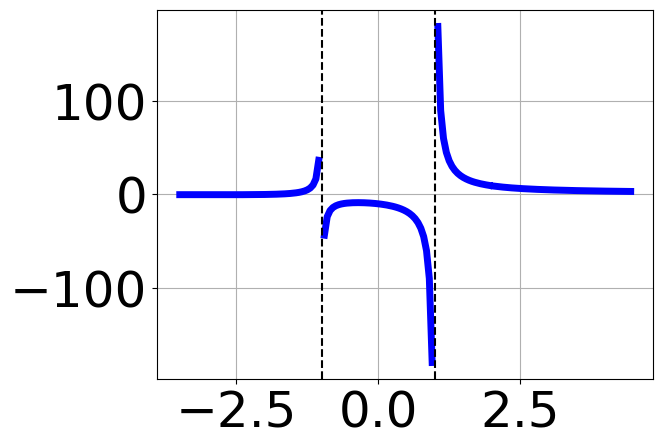
\includegraphics[width=0.5\textwidth]{../Figures/identifyGraphOfRationalFunctionCopyB.png}
\end{center}
\begin{enumerate}[label=\Alph*.]
\item \( f(x)=\frac{x^{3} -5 x^{2} -4 x + 20}{x^{3} +2 x^{2} -x -2} \)
\item \( f(x)=\frac{x^{3} + x^{2} -32 x -60}{x^{3} -2 x^{2} -x + 2} \)
\item \( f(x)=\frac{x^{3} -5 x^{2} -4 x + 20}{x^{3} +2 x^{2} -x -2} \)
\item \( f(x)=\frac{x^{3} +5 x^{2} -4 x -20}{x^{3} -2 x^{2} -x + 2} \)
\item \( \text{None of the above are possible equations for the graph.} \)

\end{enumerate} }
\litem{
Determine the vertical asymptotes and holes in the rational function below.\[ f(x) = \frac{9x^{3} -18 x^{2} -x + 10}{6x^{2} +19 x + 10} \]\begin{enumerate}[label=\Alph*.]
\item \( \text{Vertical Asymptote of } x = -2.5 \text{ and hole at } x = -0.667 \)
\item \( \text{Vertical Asymptotes of } x = -2.5 \text{ and } x = -0.667 \text{ with no holes.} \)
\item \( \text{Vertical Asymptotes of } x = -2.5 \text{ and } x = 1.667 \text{ with a hole at } x = -0.667 \)
\item \( \text{Vertical Asymptote of } x = 1.5 \text{ and hole at } x = -0.667 \)
\item \( \text{Holes at } x = -2.5 \text{ and } x = -0.667 \text{ with no vertical asymptotes.} \)

\end{enumerate} }
\litem{
Determine the vertical asymptotes and holes in the rational function below.\[ f(x) = \frac{9x^{3} +33 x^{2} -32 x -80}{6x^{2} -7 x -20} \]\begin{enumerate}[label=\Alph*.]
\item \( \text{Vertical Asymptotes of } x = 2.5 \text{ and } x = -1.333 \text{ with no holes.} \)
\item \( \text{Vertical Asymptote of } x = 1.5 \text{ and hole at } x = -1.333 \)
\item \( \text{Vertical Asymptote of } x = 2.5 \text{ and hole at } x = -1.333 \)
\item \( \text{Holes at } x = 2.5 \text{ and } x = -1.333 \text{ with no vertical asymptotes.} \)
\item \( \text{Vertical Asymptotes of } x = 2.5 \text{ and } x = 1.667 \text{ with a hole at } x = -1.333 \)

\end{enumerate} }
\end{enumerate}

\end{document}